%\documentclass[handout,xcolor=svgnames,english]{beamer}
\documentclass[xcolor=svgnames,english]{beamer}
\usetheme{DarkHU}

%\usepackage{pgfpages}
%\pgfpagesuselayout{2 on 1}[a4paper,border shrink=5mm]

% --- OPERATORS ----------------------------------------------------------------

\DeclareMathOperator{\interior}{int}
\DeclareMathOperator{\closure}{cl}
\DeclareMathOperator{\sign}{sign}
\DeclareMathOperator{\sgn}{sgn}
\DeclareMathOperator{\Div}{div}
\DeclareMathOperator{\atan}{atan2}
\DeclareMathOperator{\Curl}{Curl}
\newcommand{\conv}{\textup{conv}}
\newcommand{\Mid}{\textup{mid}}

%\DeclareMathOperator*{\liminf}{lim\,inf} % lim inf

% --- SPACES -------------------------------------------------------------------

\newcommand{\BV}{\textup{BV}}
\newcommand{\CR}{\textup{CR}}
\newcommand{\C}{\textup{C}}
\newcommand{\Vnc}{\ensuremath{V_\textup{NC}}}
% already defined\newcommand{\P}{\textup{P}}

% --- VARIABLES ----------------------------------------------------------------

\newcommand{\ucr}{u_\textup{CR}}
\newcommand{\vcr}{v_\textup{CR}}
\newcommand{\snr}{\textup{SNR}}
\newcommand{\Egleb}{E_\textup{GLEB}}

% --- FUNCTIONS ----------------------------------------------------------------

\newcommand{\Enc}{E_\textup{NC}}
\newcommand{\anc}{a_\textup{NC}}

% --- SYMBOLS/OPERATORS --------------------------------------------------------

\newcommand{\nc}{\textup{NC}}
\newcommand{\NC}{\textup{NC}}
\newcommand{\dx}{\,\mathrm{d}x}
\newcommand{\ds}{\,\mathrm{d}s}
\newcommand{\dt}{\,\mathrm{d}t}
\newcommand{\dmu}{\,\mathrm{d}\mu}
\newcommand{\gradnc}{\nabla_\textup{NC}}

% --- RELATIONS ----------------------------------------------------------------

\newcommand{\ssubset}{\subset\joinrel\subset}

% --- CALIGRAPHIC LETTERS ------------------------------------------------------

\newcommand\Acal{\mathcal{A}}
\newcommand\Bcal{\mathcal{B}}
\newcommand\Ccal{\mathcal{C}}
\newcommand\Dcal{\mathcal{D}}
\newcommand\Ecal{\mathcal{E}}
\newcommand\Fcal{\mathcal{F}}
\newcommand\Gcal{\mathcal{G}}
\newcommand\Hcal{\mathcal{H}}
\newcommand\Ical{\mathcal{I}}
\newcommand\Jcal{\mathcal{J}}
\newcommand\Kcal{\mathcal{K}}
\newcommand\Lcal{\mathcal{L}}
\newcommand\Mcal{\mathcal{M}}
\newcommand\Ncal{\mathcal{N}}
\newcommand\Ocal{\mathcal{O}}
\newcommand\Pcal{\mathcal{P}}
\newcommand\Qcal{\mathcal{Q}}
\newcommand\Rcal{\mathcal{R}}
\newcommand\Scal{\mathcal{S}}
\newcommand\Tcal{\mathcal{T}}
\newcommand\Ucal{\mathcal{U}}
\newcommand\Vcal{\mathcal{V}}
\newcommand\Wcal{\mathcal{W}}
\newcommand\Xcal{\mathcal{X}}
\newcommand\Ycal{\mathcal{Y}}
\newcommand\Zcal{\mathcal{Z}}

% --- MATHBB LETTERS -----------------------------------------------------------

\newcommand\Abb{\mathbb{A}}
%\newcommand\Bbb{\mathbb{B}}
\newcommand\Cbb{\mathbb{C}}
\newcommand\Dbb{\mathbb{D}}
\newcommand\Ebb{\mathbb{E}}
\newcommand\Fbb{\mathbb{F}}
\newcommand\Gbb{\mathbb{G}}
\newcommand\Hbb{\mathbb{H}}
\newcommand\Ibb{\mathbb{I}}
\newcommand\Jbb{\mathbb{J}}
\newcommand\Kbb{\mathbb{K}}
\newcommand\Lbb{\mathbb{L}}
\newcommand\Mbb{\mathbb{M}}
\newcommand\Nbb{\mathbb{N}}
\newcommand\Obb{\mathbb{O}}
\newcommand\Pbb{\mathbb{P}}
\newcommand\Qbb{\mathbb{Q}}
\newcommand\Rbb{\mathbb{R}}
\newcommand\Sbb{\mathbb{S}}
\newcommand\Tbb{\mathbb{T}}
\newcommand\Ubb{\mathbb{U}}
\newcommand\Vbb{\mathbb{V}}
\newcommand\Wbb{\mathbb{W}}
\newcommand\Xbb{\mathbb{X}}
\newcommand\Ybb{\mathbb{Y}}
\newcommand\Zbb{\mathbb{Z}}

% --- INTEGRAL MEAN ------------------------------------------------------------

\def\Xint#1{\mathchoice
{\XXint\displaystyle\textstyle{#1}}%
{\XXint\textstyle\scriptstyle{#1}}%
{\XXint\scriptstyle\scriptscriptstyle{#1}}%
{\XXint\scriptscriptstyle\scriptscriptstyle{#1}}%
\!\int}
\def\XXint#1#2#3{{\setbox0=\hbox{$#1{#2#3}{\int}$}
\vcenter{\hbox{$#2#3$}}\kern-.5\wd0}}
\newcommand{\intmean}{\Xint-}

% --- PERFECT BULLET -----------------------------------------------------------

\let\oldbullet\bullet
\newlength{\raisebulletlen}
\setbox1=\hbox{$\bullet$}\setbox2=\hbox{\tiny$\bullet$}
\setlength{\raisebulletlen}{\dimexpr0.5\ht1-0.5\ht2}
\renewcommand\bullet{\raisebox{\raisebulletlen}{\,\tiny$\oldbullet$}\,}
 
% --- AMSTHM ENVIRONMENtS ------------------------------------------------------

\theoremstyle{plain}
\newtheorem{theorem}{Theorem}[chapter]
\newtheorem{lemma}[theorem]{Lemma}
\newtheorem{corollary}[theorem]{Corollary}

\theoremstyle{definition}
\newtheorem{definition}[theorem]{Definition}

\theoremstyle{remark}
\newtheorem{remark}[theorem]{Remark}
 

\usepackage[backend=biber, style = alphabetic]{biblatex}
\usepackage{csquotes} % to fix biblatex warning expecting csquotes
\addbibresource{sourcesBergmannBT.bib}


\usepackage[T1]{fontenc}
\usepackage{lmodern}

\usepackage{datatool}

%\usepackage{eurosym}

%\usepackage[backend=biber, style=authortitle-icomp]{biblatex}
%\usepackage[babel,english=guillemets]{csquotes}
%\addbibresource{bib.bib}

%\usepackage{algorithm}
%\usepackage{algpseudocode}

\usepackage{tikz}
%\usetikzlibrary{shapes, fit, positioning}
%\usepackage{hyperref}

%%%%%%%%%%%%%%%%%%%%%%%
% UTF-8 input encoding
\usepackage[utf8]{inputenc}
\usepackage{microtype}\usepackage{blindtext}

% Page layout formating of koma-script
\usepackage[automark]{scrpage2}
\usepackage{lmodern}

% Language support
\usepackage[english]{babel}

% AMSMath package
\usepackage{amsmath}
\usepackage{amsfonts}
\usepackage{amssymb}
\usepackage{amstext}
\usepackage{amsopn}
\usepackage{amsthm}
\usepackage{url}
\usepackage{listings}
\usepackage{xspace}
\usepackage{mathabx}
%\usepackage{mathptmx}
\usepackage{esint}
\usepackage{mathtools}
\usepackage{hyperref}

\usepackage{subcaption}
%%%%%%%%%%%%%%%%%%%%%%%%%
\usepackage{enumitem,amssymb}
\newlist{todolist}{itemize}{2}
\setlist[todolist]{label=$\square$}
\usepackage{pifont}
\newcommand{\cmark}{\ding{51}}%
\newcommand{\xmark}{\ding{55}}%
\newcommand{\done}{\rlap{$\square$}{\raisebox{2pt}{\large\hspace{1pt}\cmark}}%
\hspace{-2.5pt}}
\newcommand{\wontfix}{\rlap{$\square$}{\large\hspace{1pt}\xmark}}
%%%%%%%%%%%%%%%%%%%%%%%%%%%


\parindent 0ex


\providecommand{\integral}[3]{\ensuremath{\int\limits_{#1} \! {#2} \, \mathrm{d}#3}}
\providecommand{\T}{\ensuremath{\mathcal{T}}}
\providecommand{\Hh}{\ensuremath{\mathrm{H}}}
\providecommand{\Ll}{\ensuremath{\mathrm{L}}}
 
%%%%%%%%%%
\setbeamercolor{green box}{use=base, fg=base.fg, bg=green}
\newenvironment{question}[1][center]{\begin{beamercolorbox}[#1, rounded=true,
  sep=1pt]{green box}}{\end{beamercolorbox}}

\setbeamercolor{yellow box}{use=base, fg=base.fg, bg=yellow}
\newenvironment{emphbox}[1][center]{\begin{beamercolorbox}[#1, rounded=true,
  sep=1pt]{yellow box}}{\end{beamercolorbox}}

\renewcommand{\emph}[1]{\textcolor{magenta}{\bfseries #1}}
\providecommand{\abs}[1]{\ensuremath{\left\lvert#1\right\rvert}}

%\setbeamercovered{transparent}
%\setbeamertemplate{navigation symbols}{}

%\expandafter\def\expandafter\insertshorttitle\expandafter{%
%  \insertshorttitle\hfill%
%    \insertframenumber\,/\,\inserttotalframenumber}

%\addtobeamertemplate{navigation symbols}{}{%
%  \usebeamerfont{footline}%
%  \usebeamercolor[fg]{footline}%
%  \hspace{1em}%
%  \insertframenumber/\inserttotalframenumber}

%\expandafter\def\expandafter\insertshorttitle\expandafter{%
%  \insertshorttitle\hfill%
%    \insertframenumber\,/\,\inserttotalframenumber}

%%%%%%%%%%%%%%%%%%%%%%%%%%%%%%%%%%%%%%%%%%%%%%%%%%%%%%%%%%%%
\author{Enrico Bergmann}
\title{The Crouzeix-Raviart Finite Element Method for a Nonconforming
Formulation of the Rudin-Osher-Fatemi Model Problem}
\institute{Humboldt-Universität zu Berlin}
\date{June 16, 2021}
\titlegraphic{
\includegraphics[height=1.6cm]{hukombi_bbw_rgb_op}}
%%%%%%%%%%%%%%%%%%%%%%%%%%%%%%%%%%%%%%%%%%%%%%%%%%%%%%%%%%%%

\usepackage{microtype}

\begin{document}

\begin{frame}[plain, noframenumbering]
	\maketitle
\end{frame}
  
\begin{frame}{Table of Contents}
  \tableofcontents
\end{frame}

%%%%%%%%%%%%%%%%%%%%%%%%%%%%%%%%%%%%%%%%%%%%%%%%%%%%%%%%%%%%%%%%%%%%%%%%%%%%%%

\section{Recapitulation}
\subsection{Functions of Bounded Variation}
\begin{frame}[noframenumbering]{Table of Contents}
  \tableofcontents[currentsection, currentsubsection]
\end{frame}

\begin{frame}
  Let $U$ be an open subset of $\Rbb^d$. A function $v\in L^1(U)$ is a function
  of bounded variation iff
  \begin{align*}
    |v|_{\BV(U)}
    \coloneqq
    \sup_{\substack{\phi\in C^1_C(U;\Rbb^d)\\
    \Vert\phi\Vert_{L^\infty(U)}\leq 1}}\int_U v\Div (\phi)\dx
    <
    \infty.
  \end{align*}
  The space of all such functions is denoted by $\BV(U)$.
  \pause
  It is a Banach space equipped with the norm $\Vert \bullet
  \Vert_{\BV(U)} \coloneqq \Vert \bullet\Vert_{L^1(U)} + |\bullet|_{\BV(U)}$.

  \pause
  \medskip
  We have $W^{1,1}(\Omega)\subset\BV(\Omega)$ with $\Vert v\Vert_{\BV(\Omega)}=
  \Vert v\Vert_{W^{1,1}(\Omega)}$ for all $v\in W^{1,1}(\Omega)$.
\end{frame}

\begin{frame}
  \fullcite{ABM14}

  \bigskip

  \fullcite{EG92}
\end{frame}

\subsection{Rudin-Osher-Fatemi Model Problem}
\begin{frame}[noframenumbering]{Table of Contents}
  \tableofcontents[currentsection, currentsubsection]
\end{frame}

\begin{frame}
  Let $\Omega\subset\Rbb^2$ be a bounded polygonal Lipschitz domain.
  \begin{block}{Rudin-Osher-Fatemi (ROF) model problem}
    For a parameter $\alpha\in \Rbb_+$ and an input signal $g\in L^2(\Omega)$
    minimize the functional
    \begin{align*}
      I(v)
      \coloneqq 
      {\color<4>{red}{|v|_{\BV(\Omega)}}}
      +\frac{\alpha}{2}
      {\color<3>{red}{\Vert v-g\Vert_{L^2(\Omega)}^2}}
    \end{align*}
    amongst all $v\in\BV(\Omega)\cap L^2(\Omega)$.
  \end{block}

  \bigskip
  \pause
  \fullcite{ROF92}
\end{frame}

\begin{frame}
  \begin{figure}[!ht]
    \centering
    \begin{subfigure}{.4\linewidth}
      \caption*{Original picture$^0$}
      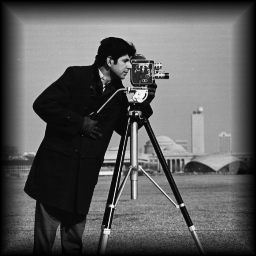
\includegraphics[width=\linewidth]
        {pictures/recap/denoiseExample/cameraman.png}
    \end{subfigure}
    \quad
    \uncover<2->{
    \begin{subfigure}{.4\linewidth}
      \caption*{Input signal}
      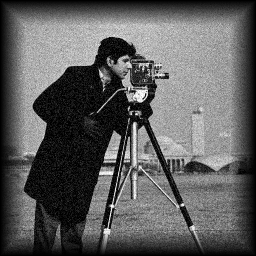
\includegraphics[width=\linewidth]
        {pictures/recap/denoiseExample/snr20.png}
    \end{subfigure}}
  \end{figure}
  \footnotetext{
  \url{https://homepages.cae.wisc.edu/~ece533/images/cameraman.tif}}
\uncover<2->{The input signal was created by adding AWGN with a SNR of 20 to
the original picture.}
\end{frame}

\begin{frame}
  \vspace{-4mm}
    \begin{align*}
      I(v)
      \coloneqq 
      {\color<3>{red}{|v|_{\BV(\Omega)}}}
      +\frac{\alpha}{2}
      {\color<2>{red}{\Vert v-g\Vert_{L^2(\Omega)}^2}}
    \end{align*}
  \vspace{-7mm}
  \begin{figure}[!ht]
    \centering
    \begin{subfigure}{.3\linewidth}
      \caption*{Original picture}
      \vspace{-2mm}
      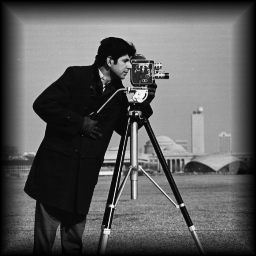
\includegraphics[width=\linewidth]
        {pictures/recap/denoiseExample/cameraman.png}
    \end{subfigure}
    \quad
    \begin{subfigure}{.3\linewidth}
      \caption*{Input signal}
      \vspace{-2mm}
      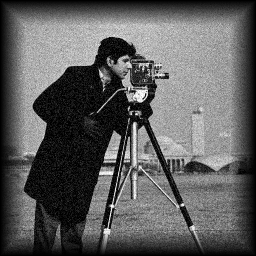
\includegraphics[width=\linewidth]
        {pictures/recap/denoiseExample/snr20.png}
    \end{subfigure}
  
    \vspace{3mm}
    \uncover<3->{
    \begin{subfigure}{.3\linewidth}
      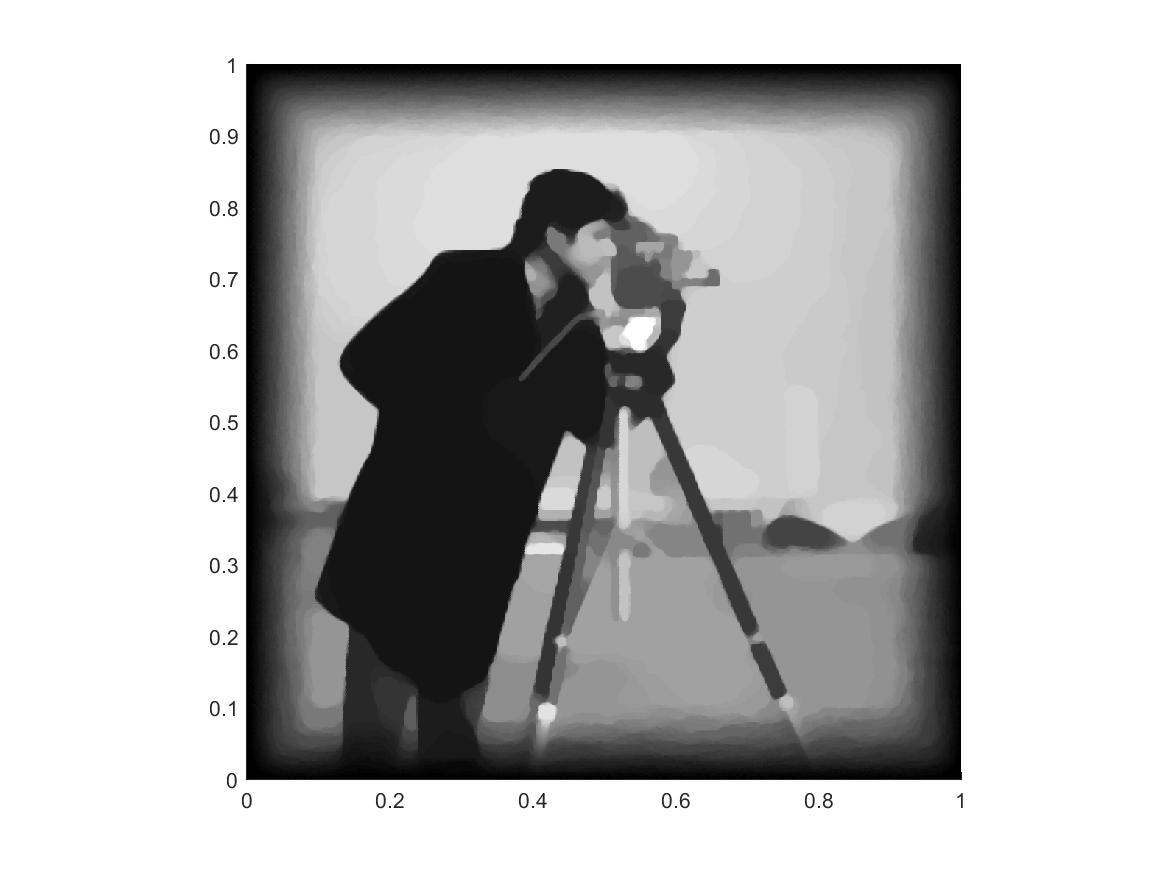
\includegraphics[trim = 60 20 60 20, clip, width=\linewidth]
        {pictures/recap/denoiseExample/alpha1e3.png}
      \caption*{$\alpha=10^3$}
    \end{subfigure}}
    \uncover<4->{
    \begin{subfigure}{.3\linewidth}
      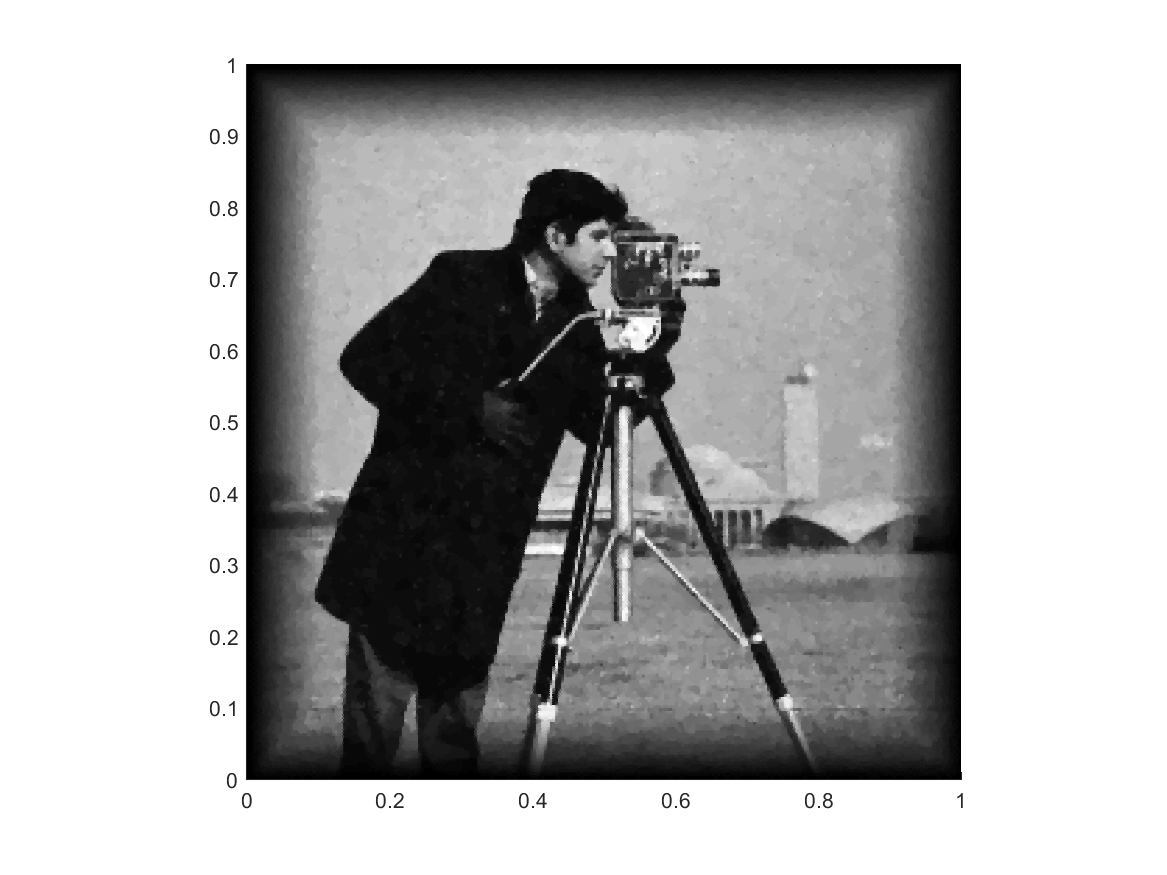
\includegraphics[trim = 60 20 60 20, clip, width=\linewidth]
        {pictures/recap/denoiseExample/alpha1e4.png}
      \caption*{$\alpha=10^4$}
    \end{subfigure}}
    \uncover<2->{
    \begin{subfigure}{.3\linewidth}
      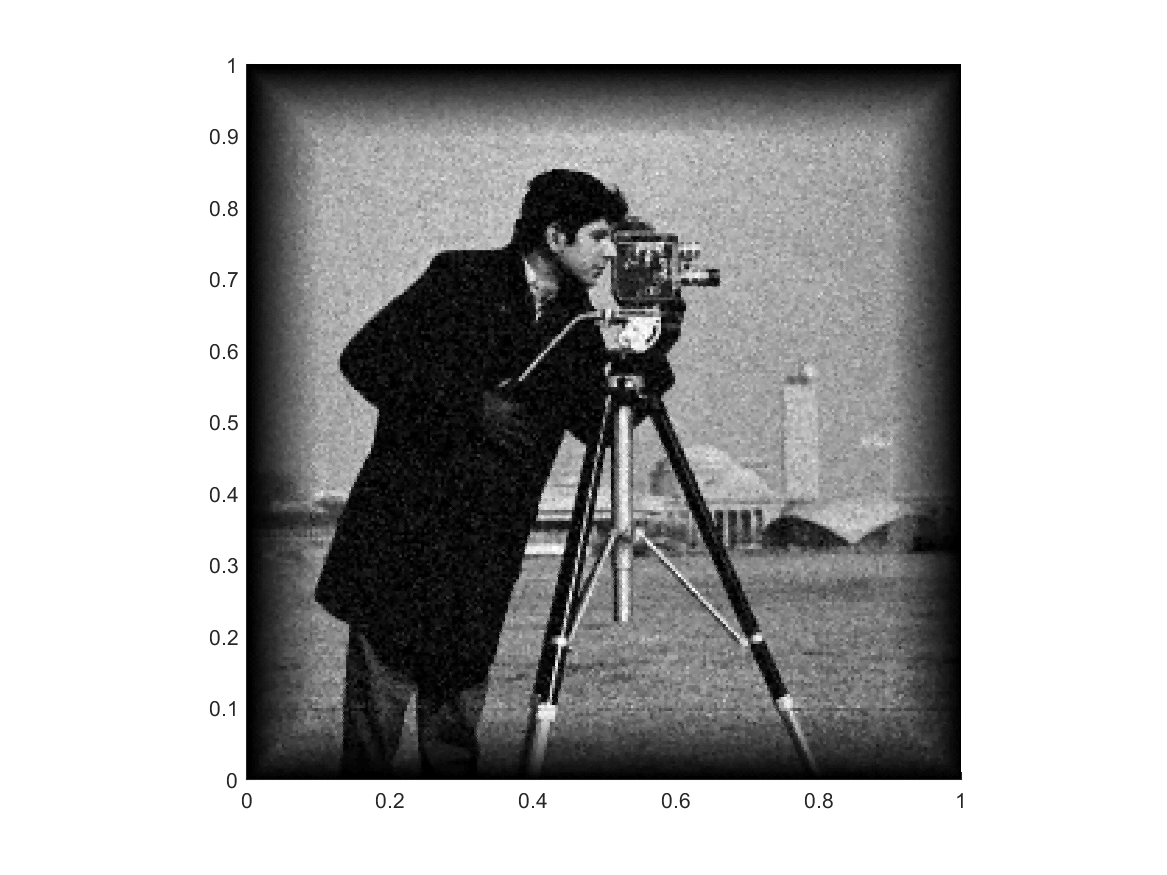
\includegraphics[trim = 60 20 60 20, clip, width=\linewidth]
        {pictures/recap/denoiseExample/alpha1e5.png}
      \caption*{$\alpha=10^5$}
    \end{subfigure}}
  \end{figure}
\end{frame}

\begin{frame}
  \fullcite{Get12}
\end{frame}

\subsection{Continuous Problem}
\begin{frame}[noframenumbering]{Table of Contents}
  \tableofcontents[currentsection, currentsubsection]
\end{frame}

\begin{frame}
  \begin{block}{Continuous problem}
    For a parameter $\alpha\in \Rbb_+$ and an input signal $f\in L^2(\Omega)$
    minimize the functional
    \begin{align*}\label{eq:continuousProblem}
      E(v)\coloneqq \frac{\alpha}{2}\Vert v\Vert^2 
      + |v|_{\BV(\Omega)} 
      + {\color<2>{red}{\Vert v\Vert_{L^1(\partial\Omega)}}}
      - \int_\Omega fv\dx
    \end{align*}
    amongst all $v\in\BV(\Omega)\cap L^2(\Omega)$.
  \end{block}

  \bigskip
  \uncover<3->{
  For $f=\alpha g$ the functional $E$ has the same minimizers as
  \begin{align*}
    I(v)
    = 
    |v|_{\BV(\Omega)}
    +\frac{\alpha}{2}
    \Vert v-g\Vert_{L^2(\Omega)}^2
  \end{align*}
  in $\left\{v\in\BV(\Omega)\cap L^2(\Omega) \mid \Vert
  v\Vert_{L^1(\partial\Omega)}=0\right\}$.}
\end{frame}

\begin{frame}
  \begin{theorem}[Existence and uniqueness]
    There exists a unique minimizer $u\in\BV(\Omega)\cap L^2(\Omega)$ for
    $E=\frac{\alpha}{2}\Vert v\Vert^2 
      + {\color<2>{red}{|v|_{\BV(\Omega)} 
      + \Vert v\Vert_{L^1(\partial\Omega)}}}
      - \int_\Omega fv\dx$ in 
     $v\in\BV(\Omega)\cap L^2(\Omega)$.
  \end{theorem}

  \pause
  \medskip
  \begin{lemma}
    Let $v\in\BV(\Omega)$.
    For all $x\in\Rbb^d$, define
    \begin{align*}
      \tilde{v}(x)\coloneqq
      \begin{cases}
        v(x)  &\text{if } x\in\Omega,\\
        0     &\text{if } x\in\Rbb^d\setminus\overline\Omega.
      \end{cases} 
    \end{align*}
    Then $\tilde{v}\in\BV\!\left(\Rbb^d\right)$ and
    $\left|\tilde{v}\right|_{\BV\!\left(\Rbb^d\right)}
    = |v|_{\BV(\Omega)}+\Vert v\Vert_{L^1(\partial\Omega)}$.
  \end{lemma}
\end{frame}


\begin{frame}
  Let $U$ be an open subset of $\Rbb^d$.

  \begin{definition}[Weak convergence in $\BV(U)$]
    Let $(v_n)_{n\in\Nbb}\subset \BV(U)$ and $v\in \BV(U)$ with
    $v_n\rightarrow v$ in $L^1(U)$ as $n\rightarrow\infty$.
    Then $(v_n)_{n\in\Nbb}$ converges weakly to $v$ in $\BV(U)$ iff,
    for all $\phi\in C_0(U;\Rbb^d)$, it holds
    \begin{align*}
      \int_U v_n\Div(\phi)\dx\rightarrow \int_U v\Div(\phi)\dx 
      \quad\text{as } n\to\infty. 
    \end{align*}
    We write $v_n\rightharpoonup v$ as $n\to\infty$.
  \end{definition}
\end{frame}

\begin{frame}
  \begin{theorem}
    Let $v\in L^1(U)$ and $(v_n)_{n\in\Nbb}\subset\BV(U)$ with
    $\sup_{n\in\Nbb}|v_n|_{\BV(U)}< \infty$ and
    $v_n\rightarrow v$ in $L^1(U)$ as $n\rightarrow\infty$.
    Then $v\in\BV(U)$ and $|v|_{\BV(U)}\leq
    \liminf_{n\rightarrow\infty}|v_n|_{\BV(U)}.$
    Furthermore, $v_n\rightharpoonup v$ in $\BV(U)$.
  \end{theorem}

  \pause
  \medskip
  Let $U$ be a bounded Lipschitz domain.
  
  \begin{theorem}[\protect{\cite[S. 176, Theorem 4]{EG92}}]
    \label{thm:l1ConvergentSubsequence}
    Let $(v_n)_{n\in\Nbb}\subset \BV(U)$ be bounded. Then
    there exists some subsequence $(v_{n_k})_{k\in\Nbb}$ of
    $(v_n)_{n\in\Nbb}$ and $v\in\BV(U)$ such that
    $v_{n_k}\to v$ in $L^1(U)$ as $k\to \infty$.
  \end{theorem}
\end{frame}

\begin{frame}
  \begin{block}{Stability}
    Let $f_1,f_2\in L^2(\Omega)$.
    For $\ell\in\{1,2\}$, let $u_\ell\in \BV(\Omega)\cap L^2(\Omega)$ minimize
    \begin{align*}
      E_\ell
      \coloneqq 
      {\color<3>{red}{\frac{\alpha}{2}\Vert v\Vert^2}}
      + {\color<4>{red}{|v|_{\BV(\Omega)} 
      + \Vert v\Vert_{L^1(\partial\Omega)} }}
      {\color<3>{red}{- \int_\Omega f_\ell v\dx}}
    \end{align*}
    amongst all $v\in\BV(\Omega)\cap L^2(\Omega)$.
    Then
    \begin{align*}
      \Vert u_1 - u_2\Vert 
      \leq\frac{1}{\alpha}\Vert f_1-f_2\Vert.
    \end{align*}
  \end{block}

  \medskip
  \pause
  \fullcite[Chapter 10]{Bar15}.

\end{frame}

\subsection{Discrete Problem}
\begin{frame}[noframenumbering]{Table of Contents}
  \tableofcontents[currentsection, currentsubsection]
\end{frame}

\begin{frame}
  nochmal Existenz und Eindeutigkeitsaussagen zeigen und gaaaanz grob 
  beschreiben, wie die bewiesen werden
\end{frame}

\subsection{Discrete Problem continues}
\begin{frame}[noframenumbering]{Table of Contents}
  \tableofcontents[currentsection, currentsubsection]
\end{frame}

\begin{frame}
  vielleicht in eigener Section: noch die Aussagen aus der Arbeit verarbeiten,
  die über Existenz und Eindeutigkeit hinausgehen
\end{frame}


\begin{frame}
  \fullcite[Chapter 10, p. 297-319]{Bar15}
\end{frame}

\begin{frame}{Properties of $\BV(\Omega)$}
\end{frame}

\begin{frame}{Notions of convergence on $\BV(\Omega)$}
  Let $(v_n)_{n\in\Nbb}\subset \BV(\Omega)$ and $v\in \BV(\Omega)$ such that
  $v_n\rightarrow v$ in $L^1(\Omega)$ as $n\rightarrow\infty$.
  \pause
  \begin{itemize}
    \item[(i)]
      $(v_n)_{n\in\Nbb}$ converges intermediately or strictly to $v$
      if $|v_n|_{\BV(\Omega)}\rightarrow |v|_{\BV(\Omega)}$ as
      $n\rightarrow\infty$.
      \pause
    \item[(ii)] $(v_n)_{n\in\Nbb}$ converges weakly to
      $v$ if
      $\langle Dv_n,\phi\rangle\rightarrow \langle Dv,\phi\rangle$ 
      for all $\phi\in C_0(\Omega;\Rbb^n)$ as 
      $n\rightarrow\infty$.
  \end{itemize}
\end{frame}

\begin{frame}{Further Properties of $\BV(\Omega)$}
  $C^\infty(\overline\Omega)$ and $C^\infty(\Omega)\cap\BV(\Omega)$ are dense
  in $\BV(\Omega)$ with respect to intermediate convergence.
  
  \pause
  \bigskip

  The embedding $\BV(\Omega)\to L^p(\Omega)$ is continuous for
  $1\leq p\leq n/(n-1)$ and compact for $1\leq p< n/(n-1)$.
  
  \pause
  \bigskip

  There exists a linear operator $T:\BV(\Omega)\to L^1(\partial\Omega)$
  such that $T(v) = v|_{\partial\Omega}$ for all $v\in\BV(\Omega)\cap
  C(\overline\Omega)$.

  $T$ is continuous with respect to intermediate convergence in $\BV(\Omega)$
  but not with respect to weak convergence in $\BV(\Omega)$. 
\end{frame}



\section{Primal-Dual Iteration}
\begin{frame}[noframenumbering]{Table of Contents}
  \tableofcontents[currentsection, currentsubsection]
\end{frame}

\begin{frame}
  \begin{algorithm}[Primal-dual iteration]
  \begin{algorithmic}
    \Require $\left(u_0,\Lambda_0\right)
    \in\textup{CR}_0^1(\mathcal{T})\times P_0\!\left(\mathcal{T}; 
    %\left\{w\in\Rbb^2\,\middle|\,|w|\leq 1\right\}\right),
    \overline{B_{\Rbb^2}}\right)$, 
    %\overline{B_1(0)}\right),
    \pause$\tau>0$\only<12>{, {\color{red}$\varepsilon_\textup{stop}>0$}}  \\
    \pause Initialize $v_0\coloneqq 0$ in $\textup{CR}^1_0(\mathcal T)$.
    \pause\For{$j = 1,2,\dots$}
    \begin{align*}
      \tilde{u}_j&\coloneqq u_{j-1}+\tau v_{j-1},
      &&&\Lambda_j
      &\coloneqq
      \frac{\Lambda_{j-1}+\tau\nabla_{\textup{NC}} \tilde{u}_j}
      {\max\left\{1,
      \left|\Lambda_{j-1}+\tau\nabla_{\textup{NC}}\tilde{u}_j\right|\right\}},
    \end{align*}
    \pause\State solve  % TODO habe Antwort parat für ,,Was ist diese Gleichung
    \begin{align*}
      \label{eq:linSysPrimalDualAlg}
      \frac{1}{\tau}{\color<8,10-11>{red}{a_{\textup{NC}}(u_j,\bullet)}}
      +\alpha{\color<9>{red}{(u_j,\bullet)}}
      &=
      \frac{1}{\tau}{\color<10-11>{red}{a_{\textup{NC}}(u_{j-1},\bullet)}} 
      + (f,\bullet)
      - \left(\Lambda_j,\nabla_{\textup{NC}}\bullet\right) 
    \end{align*}
    \State in $\CR^1_0(\Tcal)$ for $u_j$, \pause and set
    \begin{equation*}
      {\color<11>{green}{v_j\coloneqq\frac{u_j-u_{j-1}}{\tau}}}.
      {\only<12>{\color{red}\text{ Terminate iteration if }\vvvert v_j\vvvert<
      \varepsilon_\textup{stop}.}}
    \end{equation*}
    \EndFor
    \pause\Ensure Sequence $(u_j,\Lambda_j)_{j\in\mathbb N}$ in
    $\CR^1_0(\mathcal{T})\times
     P_0\!\left(\mathcal{T};\overline{B_{\Rbb^2}}\right)$   
    \end{algorithmic}
  \end{algorithm}
\end{frame}

\begin{frame}
  \begin{theorem}[Convergence of the primal-dual iteration]
    Let $\ucr\in \CR^1_0(\Tcal)$ solve the discrete problem,
    $\bar\Lambda_0\in P_0\!\left(\Tcal;\Rbb^2\right)$ satisfy
    $\left|\bar\Lambda_0(\bullet)\right|\leq 1$ a.e.\ in $\Omega$ as well as
    \begin{equation*}
      \bar\Lambda_0(\bullet)\cdot\gradnc\ucr(\bullet)
      =
      \left|\gradnc\ucr(\bullet)\right| 
      \quad\text{a.e.\ in } \Omega 
    \end{equation*}
    and
    \begin{equation*}
      \left(\bar\Lambda_0,\gradnc\vcr\right)
      = \left(f-\alpha\ucr,
      \vcr\right)
      \quad\text{for all } \vcr\in\CR^1_0(\Tcal),
    \end{equation*}
    and {\color<3>{red}{$\tau \in (0, 1]$}}.
    Then the iterates $(u_j)_{j\in\Nbb}$ of
    the primal-dual iteration converge to $\ucr$ in $L^2(\Omega)$.
  \end{theorem}

  \pause
  \medskip

  \only<-3>{For all $J\in\Nbb$,} 
  \begin{align*}
    \sum_{j=1}^{\only<-3>{J}\only<4->{\infty}}\Vert \ucr-u_j\Vert^2 
    \leq
    \frac{1}{2\alpha{\color<3>{red}{\tau}}}
    \left(\vvvert \ucr-u_0\vvvert^2_\nc 
    + \Vert \bar\Lambda_0-\Lambda_0\Vert^2\right).
  \end{align*}
\end{frame}


\section{Numerical Examples}
\section{Konstruktion eines Experiments mit exakter Lösung}
Um eine rechte Seite zu finden, zu der die exakte Lösung bekannt
ist, wähle eine Funktion des Radius $u\in H^1_0([0,1])$ mit Träger im 
zweidimensionalen Einheitskreis. Insbesondere muss damit gelten $u(1)=0$ und
$u$ stetig.
Die rechte Seite als Funktion des Radius $f\in L^2([0,1])$ ist dann gegeben
durch 
\begin{align*}
  f \coloneqq 
  \alpha u - \partial_r(\sign(\partial_r u)) - \frac{\sign(\partial_r u)}{r},
\end{align*}
wobei für $F\in\Rbb^2\setminus\{0\}$ gilt 
$\sign(F)\coloneqq \left\{\frac{F}{|F|}\right\}$ 
und $\sign(0)\in B_1(0)$.
Damit außerdem gilt $f\in H^1_0([0,1])$, was z.B.\ für GLEB relevant ist, 
muss also noch Stetigkeit von $\sign(\partial_r u)$ und 
$\partial_r(\sign(\partial_r u))$ verlangt werden und 
$\partial_r(\sign(\partial_r u(1))=\sign(\partial_r u(1))=0$.
Damit $f$ in $0$ definierbar ist, muss auch gelten 
$\sign(\partial_r u) \in o(r)$ für $r\to 0$.

Damit erhält man für die Funktion
\begin{align*}
  u_1(r)\coloneqq
  \begin{cases}
    1, & \text{wenn } 0\leq r\leq\frac{1}{6},\\
    1+(6r-1)^\beta, & \text{wenn } \frac{1}{6}\leq r\leq\frac{1}{3},\\
    2, &\text{wenn } \frac{1}{3}\leq r\leq\frac{1}{2},\\
    2(\frac{5}{2}-3r)^\beta, &\text{wenn } \frac{1}{2}\leq r\leq\frac{5}{6},\\
    0, &\text{wenn } \frac{5}{6}\leq r,
  \end{cases}
\end{align*}
wobei $\beta\geq 1/2$, mit der Wahl
\begin{align*}
  \sign(\partial_r u_1(r)) =
  \begin{cases}
    12r-36r^2, & \text{wenn } 0\leq r\leq\frac{1}{6},\\
    1, & \text{wenn } \frac{1}{6}\leq r\leq\frac{1}{3},\\
    \cos(\pi(6r-2)), &\text{wenn } \frac{1}{3}\leq r\leq\frac{1}{2},\\
    -1, &\text{wenn } \frac{1}{2}\leq r\leq\frac{5}{6},\\
    -\frac{1+\cos(\pi(6r-5))}{2}, &\text{wenn } \frac{5}{6}\leq r\leq 1,
  \end{cases}
\end{align*}
die rechte Seite
\begin{align*}
  f_1(r)\coloneqq 
  \begin{cases}
    \alpha-12(2-9r), & \text{wenn } 0\leq r\leq\frac{1}{6},\\
    \alpha(1+(6r-1)^\beta)-\frac{1}{r}, & \text{wenn } \frac{1}{6}\leq r\leq
    \frac{1}{3},\\
    2\alpha+6\pi\sin(\pi(6r-2))-\frac{1}{r}\cos(\pi(6r-2)), &
    \text{wenn } \frac{1}{3}\leq r\leq\frac{1}{2},\\
    2\alpha(\frac{5}{2}-3r)^\beta+\frac{1}{r},&
    \text{wenn } \frac{1}{2}\leq r\leq\frac{5}{6},\\
    -3\pi\sin(\pi(6r-5))+\frac{1+\cos(\pi(6r-5))}{2r}, &
    \text{wenn } \frac{5}{6}\leq r\leq 1.
  \end{cases}
\end{align*}

Für die Funktion
\begin{align*}
  u_2(r)\coloneqq 
  \begin{cases}
    1, & \text{wenn } 0\leq r\leq\frac{1-\beta}{2},\\
    -\frac{1}{\beta}r + \frac{1+\beta}{2\beta}, & 
    \text{wenn } \frac{1-\beta}{2}\leq r\leq \frac{1+\beta}{2},\\
    0, & \text{wenn } \frac{1+\beta}{2}\leq r,
  \end{cases}
\end{align*}
erhält man mit der Wahl
\begin{align*}
  \sign&(\partial_r u_2(r)) \\
  &\coloneqq 
  \begin{cases}
    \frac{4}{1-\beta}r\left(\frac{1}{1-\beta}r -1\right), &
    \text{wenn } 0\leq r\leq\frac{1-\beta}{2},\\
    -1, & \text{wenn } \frac{1-\beta}{2}\leq r\leq \frac{1+\beta}{2},\\
    \frac{4}{(\beta-1)^3}
    \left( 4r^3-3(\beta+3)r^2 +6(\beta+1)r-3\beta-1\right), & 
    \text{wenn } \frac{1+\beta}{2}\leq r\leq 1,
  \end{cases}
\end{align*}
die rechte Seite
\begin{align*}
  f_2(r)\coloneqq 
  \begin{cases}
    \alpha - \frac{4}{1-\beta}\left(\frac{3}{1-\beta}r - 2\right), &
    \text{wenn } 0\leq r\leq\frac{1-\beta}{2},\\
    -\frac{\alpha}{\beta}\left( r-\frac{1+\beta}{2} \right) +\frac{1}{r}, & 
    \text{wenn } \frac{1-\beta}{2}\leq r\leq \frac{1+\beta}{2},\\
    \frac{-4}{(\beta-1)^3}
    \left( 16r^2 -9(\beta+3)r + 12(\beta+1) - \frac{3\beta+1}{r}\right), & 
    \text{wenn } \frac{1+\beta}{2}\leq r\leq 1.
  \end{cases}
\end{align*}

Damit können Experimente durchgeführt werden bei denen 
\texttt{exactSolutionKnown = true} gesetzt werden kann und entsprechend auch 
der $L^2$-Fehler berechnet wird.

Soll nun auch die Differenz der exakten Energie mit der garantierten unteren 
Energie Schranke (GLEB) berechnet werden, dann werden die stückweisen
Gradienten der exakten Lösung und der rechten Seite benötigt.

Dabei gelten folgende Ableitungsregeln für die Ableitungen einer Funktion 
$g$, wenn man ihr Argument $x=(x_1,x_2)\in\Rbb^2$ in Polarkoordinaten mit Länge
$r=\sqrt{x_1^2+x_2^2}$ und Winkel
$\varphi = \atan(x_2,x_1)$, wobei 
\begin{align*}
  \atan(x_2,x_1)\coloneqq
  \begin{cases}
    \arctan\left( \frac{x_2}{x_1} \right),& \text{wenn }x_1>0,\\
    \arctan\left( \frac{x_2}{x_1} \right) +\pi,& \text{wenn }x_1<0,x_2\geq 0,\\
    \arctan\left( \frac{x_2}{x_1} \right) -\pi,& \text{wenn }x_1<0,x_2<0,\\
    \frac{\pi}{2},& \text{wenn }x_1=0,x_2>0,\\
    -\frac{\pi}{2},& \text{wenn }x_1=0,x_2<0,\\
    \text{undefiniert},& \text{wenn }x_1=x_2=0,\\
  \end{cases}
\end{align*}
auffasst,
\begin{align*}
  \partial_{x_1} &= 
  \cos(\varphi)\partial_r - \frac{1}{r}\sin(\varphi)\partial_\varphi,\\
  \partial_{x_2} &= 
  \sin(\varphi)\partial_r - \frac{1}{r}\cos(\varphi)\partial_\varphi.
\end{align*}
Ist $g$ vom Winkel $\varphi$ unabhängig, so ergibt sich
\begin{align*}
  \nabla_{(x_1,x_2)}g = (\cos(\varphi),\sin(\varphi))\partial_r g.
\end{align*}
Unter Beachtung der trigonometrischen Zusammenhänge
\begin{align*}
  \sin(\arctan(y)) = \frac{y}{\sqrt{1+y^2}},\\
  \cos(\arctan(y)) = \frac{1}{\sqrt{1+y^2}}
\end{align*}
ergibt sich 
\begin{align*}
  (\cos(\varphi),\sin(\varphi)) = (x_1,x_2)\frac{1}{r}
\end{align*}
und damit 
\begin{align*}
  \nabla_{(x_1,x_2)}g = (x_1,x_2)\frac{\partial_r g}{r},
\end{align*} 
es muss also nur $\partial_r g$ bestimmt werden.

Die entsprechenden Ableitung lauten
\begin{align*}
  \partial_r f_1(r) &= 
  \begin{cases}
    108,&
    \text{wenn }0\leq r\leq\frac{1}{6},\\
    6\alpha\beta(6r-1)^{\beta-1} +\frac{1}{r^2}, &
    \text{wenn } \frac{1}{6}\leq r\leq\frac{1}{3},\\
    (36\pi^2+\frac{1}{r^2})\cos(\pi(6r-2))+
    \frac{6\pi}{r}\sin(\pi(6r-2)), &
    \text{wenn } \frac{1}{3}\leq r\leq\frac{1}{2},\\
    -\left(6\alpha\beta\left( \frac{5}{2}-3r \right)^{\beta-1}+
    \frac{1}{r^2}\right),&
    \text{wenn } \frac{1}{2}\leq r\leq\frac{5}{6},\\
    -\left( \left( 18\pi^2+\frac{1}{2r^2} \right)\cos(\pi(6r-5))
    +\frac{1}{2r^2}+\frac{3\pi}{r}\sin(\pi(6r-5))\right),
    &\text{wenn } \frac{5}{6}\leq r\leq 1,
  \end{cases}\\
  \partial_r u_1(r) &= 
  \begin{cases}
    0,&\text{wenn }0\leq r\leq\frac{1}{6},\\
    6\beta(6r-1)^{\beta-1}, &\text{wenn } \frac{1}{6}\leq r\leq\frac{1}{3},\\
    0, &\text{wenn } \frac{1}{3}\leq r\leq\frac{1}{2},\\
    -6\beta\left( \frac{5}{2}-3r \right)^{\beta-1},&
    \text{wenn } \frac{1}{2}\leq r\leq\frac{5}{6},\\
    0,&\text{wenn } \frac{5}{6}\leq r,
  \end{cases}\\
  \partial_r f_2(r) &= 
  \begin{cases}
    -\frac{12}{(1-\beta)^2},&\text{wenn }0\leq r\leq\frac{1-\beta}{2},\\
    -\frac{\alpha}{\beta}-\frac{1}{r^2},&
    \text{wenn } \frac{1-\beta}{2}\leq r\leq \frac{1+\beta}{2},\\
    -\frac{4}{(1-\beta)^3}\left( 32r-9(\beta+3)+\frac{3\beta+1}{r^2} \right),&
    \text{wenn } \frac{1+\beta}{2}\leq r\leq 1,\\
  \end{cases}\\
  \partial_r u_2(r) &= 
  \begin{cases}
    0,&\text{wenn }0\leq r\leq\frac{1-\beta}{2},\\
    -\frac{1}{\beta},&
    \text{wenn } \frac{1-\beta}{2}\leq r\leq \frac{1+\beta}{2},\\
    0,&\text{wenn } \frac{1+\beta}{2}\leq r.
  \end{cases}
\end{align*}

Mit diesen Informationen kann mit \texttt{computeExactEnergyBV.m} die exakte 
Energie berechnet werden und somit durch eintragen der exakten Energie
in die Variable \texttt{exactEnergy} im Benchmark und setzen der Flag
\texttt{useExactEnergy=true} das Experiment durch anschließendes Ausführen
von \texttt{startAlgorithmCR.m} gestartet werden.


\todo[inline]{Take a look at denoising and read [ROF92] for that.}


\section*{Appendix}
\begin{frame}[noframenumbering]{Table of Contents}
  \tableofcontents[currentsection, currentsubsection]

  \center{\textbf{Thank you for your attention.}}
\end{frame}
  %tien schicken spätestens am Wochenende vor der Präsi, CC vor der Präsi
  %die fertige Präsi + akuteller Stand der Arbeit schicken

\begin{frame}
  L2 Sprünge vielleicht auswerten (bleiben sie konstant\ldots, if we consider
  them, it becomes conforming

  die L2 Sprung entwicklung einiger experiment (iteration auswerten, iteration 
  selbst und Afem loop insgesamt). bleiben sicherlich konstant oder sowas
\end{frame}

\begin{frame}
  differenct norm for termination criteria comparison (energy difference not
  good because oscillations, everything else (dont show L2 error squared)
  is similar, just different height
\end{frame}

\begin{frame}
  compare times without preallocating and with (inform about the extreme 
  improvement of performance
\end{frame}

\begin{frame}
  Let $u_P:[0,\infty)\to\Rbb$ with $u_P(r)=0$ for $r\geq 1$,
  and, for all $x\in\Omega$, $u(x)= u_P\big(|x|\big)$. 
  \pause
  Furthermore, assume the existence  of $\partial_r u_P$ a.e.\ in $[0,\infty)$,
  the existence of the derivative of
  \begin{align*}
    \operatorname{sgn}\big(\partial_r u_P(r)\big)
    \coloneqq
    \begin{cases}
      -1 &\text{für }\partial_r u_P(r)<0,\\
      x\in[0,1] &\text{für }\partial_r u_P(r)=0,\\ 
      1 &\text{für }\partial_r u_P(r)>0.
    \end{cases}
  \end{align*}
  a.e.\ in $[0,\infty)$, and
  that $\operatorname{sgn}\big(\partial_r u_P(r)\big)/r\to 0$ as $r\to 0$.
  \pause
  For all $r\in[0,\infty)$, define 
  \begin{align*}
    f_P(r)
    \coloneqq 
    \alpha u_P(r) - \partial_r\left(\operatorname{sgn}\big(\partial_r u_P(r)\big)\right) 
    - \frac{\operatorname{sgn}\big(\partial_r u_P(r)\big)}{r}
  \end{align*}
  \pause
  Then $u$ solves the continuous problem
  on $\Omega\supseteq \left\{w\in\Rbb^2\,\middle|\, |w|\leq 1\right\}$ if
  the input signal is $f(x)\coloneqq f_P\big(|x|\big)$.
\end{frame}

\end{document}
